\begin{center}
    \Large\textbf{Xây dựng trang web đầu tiên với FastAPI: Hướng dẫn toàn~diện cho người mới bắt đầu}
\end{center}

\begin{center}
    \Large\textit{Trịnh Nguyễn Huy Hoàng}
\end{center}

% \begin{center}
%     \large\textit{Hành trình rủ thêm đồng bọn của Decision Tree để tạo ra "hội đồng" mạnh hơn, hiệu quả hơn trong các bài toán phân loại và hồi quy.}
% \end{center}

\begin{abstract}
Được xây dựng để giải quyết những thách thức của kỷ nguyên số, FastAPI nổi bật với tốc độ vượt trội, hiệu quả tối đa và khả năng tự động hóa đáng kinh ngạc. Bài viết này là một cẩm nang toàn diện, dẫn dắt từ những khái niệm nền tảng nhất cho đến việc xây dựng một ứng dụng web hoàn chỉnh, có tính ứng dụng cao, đặc biệt là trong lĩnh vực trí tuệ AI.
\end{abstract}

%\begin{minted}
% \tableofcontents
%\end{minted}

\section{Giới thiệu về FastAPI}
\label{sec:fastapi}

\subsection{API là gì?}

API (Application Programming Interface) là một giao diện phần mềm cho phép hai ứng dụng khác nhau giao tiếp với nhau. Có thể hình dung API như một người phục vụ tại nhà hàng: khi một người khách muốn gọi món, họ không cần phải vào bếp mà chỉ cần đưa yêu cầu cho người phục vụ. Người phục vụ sẽ nhận yêu cầu, chuyển đến bếp và mang món ăn trở lại cho khách. API cũng tương tự, nó giúp các lập trình viên sử dụng các chức năng phức tạp, chẳng hạn như dữ liệu thời tiết hoặc bản đồ, mà không cần hiểu chi tiết bên trong của hệ thống đó. Điều này cho phép chúng ta xây dựng các ứng dụng mới một cách nhanh chóng bằng cách ghép nối các "khối chức năng" (API) với nhau, giống như việc lắp ráp các viên gạch Lego.

\begin{figure}[H]
    \centering
    \includegraphics[width=\linewidth]{projects/FastAPI/image/FastAPI_1.png}
    \caption{Sơ đồ kiến trúc API với client và server}
\end{figure}

REST API (Representational State Transfer) là một kiểu thiết kế API sử dụng các phương thức HTTP tiêu chuẩn như GET, POST, PUT, DELETE để thực hiện các thao tác CRUD (Create, Read, Update, Delete) trên dữ liệu. REST API có những đặc điểm quan trọng:
\begin{itemize}[noitemsep]
\item \textbf{Stateless:} Mỗi request đều độc lập, không lưu trữ thông tin giữa các request
\item \textbf{Uniform Interface:} Sử dụng các URL để xác định resources và HTTP methods để thao tác
\item \textbf{Client-Server Architecture:} Tách biệt rõ ràng giữa client và server
\end{itemize}

\subsection{ASGI Server và Unicorn}

Trước khi FastAPI xuất hiện, hầu hết các framework web Python đều dựa trên giao thức \emph{WSGI (Web Server Gateway Interface)}, được thiết kế cho mô hình xử lý request đồng bộ. Điều này có nghĩa là khi một request đến, server sẽ xử lý nó từ đầu đến cuối trước khi có thể chấp nhận request tiếp theo. Phương pháp này không hiệu quả khi gặp các tác vụ tốn thời gian như truy vấn cơ sở dữ liệu hoặc gọi đến một API bên ngoài, vì nó sẽ làm "tắc nghẽn" toàn bộ hệ thống.   

Để khắc phục nhược điểm này, tiêu chuẩn \textit{\textbf{ASGI (Asynchronous Server Gateway Interface)}} đã ra đời, mở đường cho lập trình bất đồng bộ. FastAPI là một trong những framework tiên phong tuân thủ tiêu chuẩn này. 

Điều quan trọng cần nắm là FastAPI không phải là một máy chủ web độc lập. Thay vào đó, nó là một "ứng dụng" tuân thủ giao thức ASGI và cần một máy chủ web ASGI để chạy. Uvicorn là một máy chủ web ASGI hiệu suất cao, được tạo ra để chuyên biệt cho các ứng dụng như FastAPI.   

Uvicorn chịu trách nhiệm lắng nghe các request đến từ client và chuyển chúng đến FastAPI để xử lý. Việc tách biệt này cho phép FastAPI tập trung vào việc xử lý logic nghiệp vụ, trong khi Uvicorn đảm nhận vai trò quản lý kết nối và tối ưu hóa hiệu suất.

Sơ đồ kiến trúc của ASGI Server được minh hoạ như hình \ref{fig:fastapi2}. Cần lưu ý rằng, Uvicorn hỗ trợ HTTP/1.1 và WebSockets, cho phép xử lý nhiều request đồng thời một cách hiệu quả. Điều này đặc biệt quan trọng khi xây dựng các API cần xử lý nhiều request cùng lúc.

\begin{figure}[H]
    \centering
    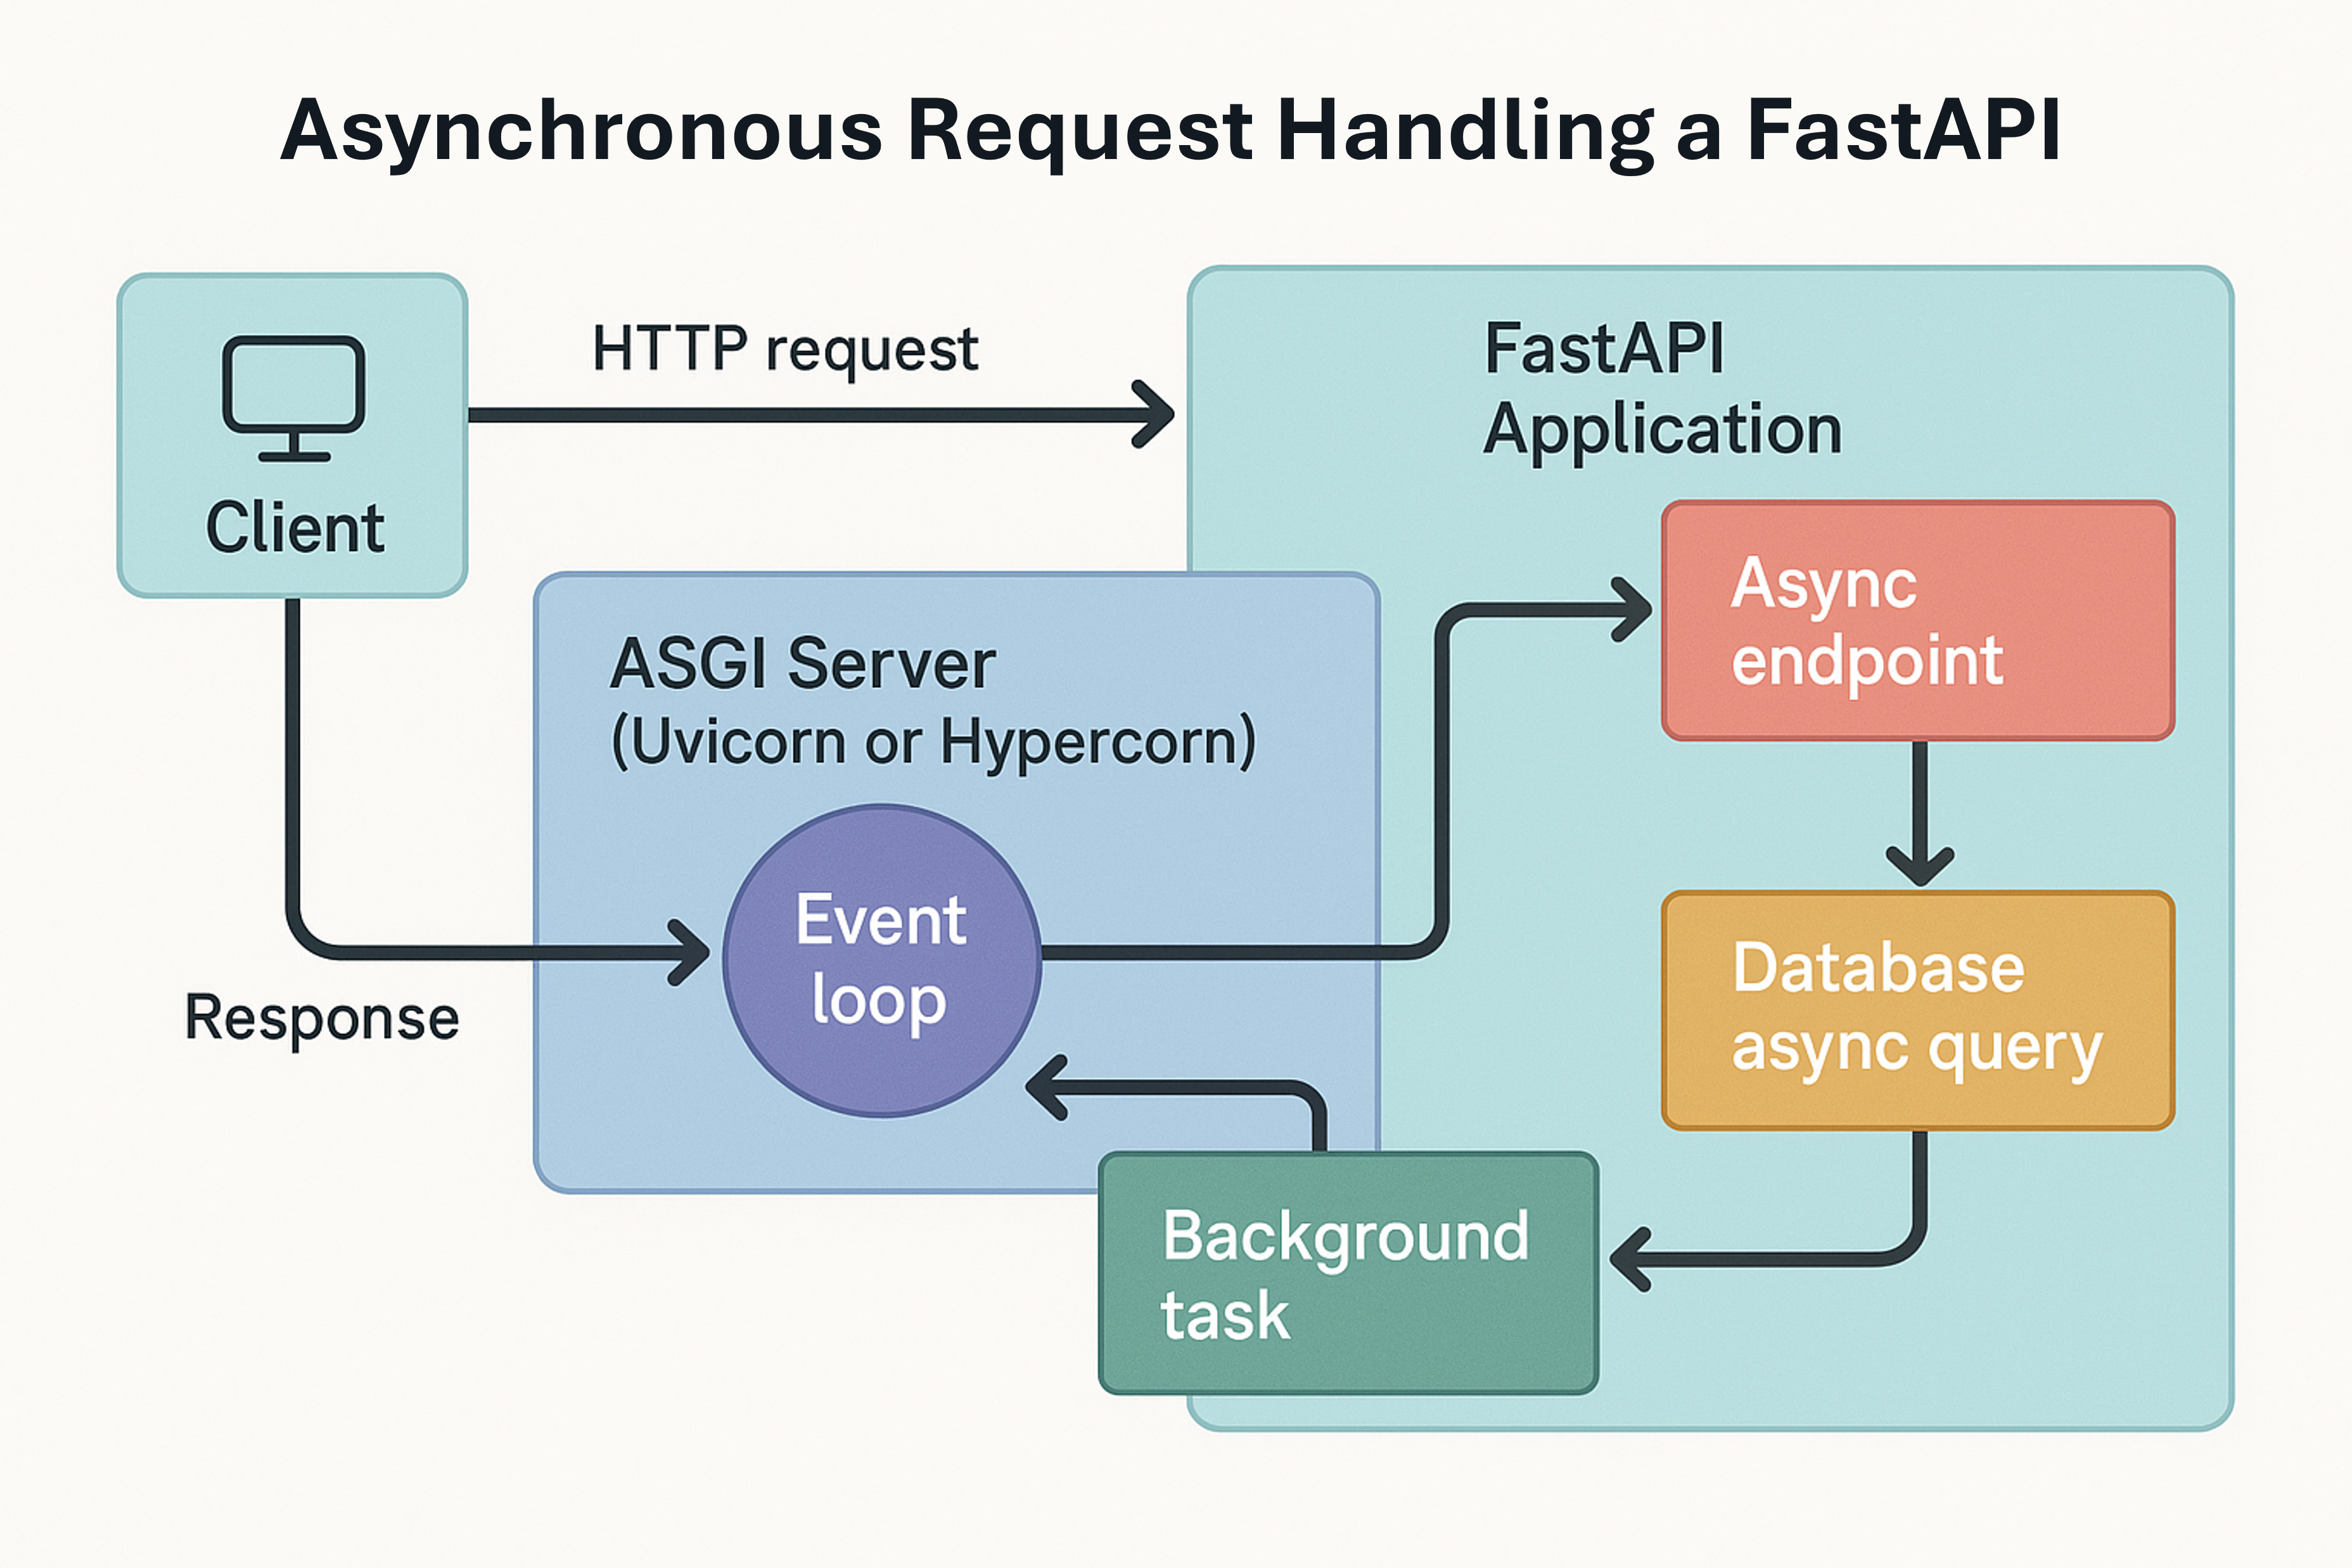
\includegraphics[width=0.7\linewidth]{projects/FastAPI/image/FastAPI_2.png}
    \caption{Sơ đồ kiến trúc ASGI server với xử lý bất đồng bộ}
    \label{fig:fastapi2}
\end{figure}

\subsection{Hiểu rõ async và await}

Lập trình bất đồng bộ là một khái niệm cốt lõi của FastAPI. Không giống như lập trình đa luồng (multi-threading) hay đa tiến trình (multi-processing), lập trình bất đồng bộ trong Python là một kỹ thuật "đơn luồng, đa tác vụ" (single-threaded, multi-tasking).   

Hãy tưởng tượng bạn đang chơi cờ với 24 người cùng một lúc. Thay vì chơi một ván cờ duy nhất từ đầu đến cuối (mô hình đồng bộ), bạn sẽ di chuyển từ bàn này sang bàn khác, thực hiện một nước cờ và ngay lập tức chuyển sang bàn tiếp theo, cho phép đối thủ của mình suy nghĩ. Tương tự, trong lập trình bất đồng bộ, khi một tác vụ I/O-bound (như truy vấn cơ sở dữ liệu hoặc chờ phản hồi từ một API khác) đang chờ, \verb|await| sẽ tạm dừng việc thực thi của hàm hiện tại và chuyển quyền điều khiển cho event loop (vòng lặp sự kiện) để xử lý các tác vụ khác.  

\begin{itemize}[noitemsep]
\item \emph{async def} được sử dụng để định nghĩa một \emph{coroutine} function, một loại hàm có thể bị tạm dừng.   
\item \emph{await} chỉ có thể được sử dụng bên trong một hàm \emph{async def} và là từ khóa để tạm dừng việc thực thi và nhường quyền điều khiển.   
\end{itemize}

Điều này cực kỳ quan trọng đối với các ứng dụng web vì phần lớn thời gian chờ đợi là do các tác vụ I/O. Bằng cách tận dụng async/await, FastAPI có thể xử lý hàng ngàn kết nối đồng thời trên một luồng duy nhất, tránh được chi phí và sự phức tạp của việc quản lý đa luồng. Chính nhờ cơ chế này, FastAPI được đánh giá là một trong những framework Python nhanh nhất, sánh ngang với Node.js và Go.

\subsection{FastAPI, Flask và Django}

Khi bắt đầu một dự án web Python, ta thường băn khoăn giữa ba lựa chọn phổ biến: Django, Flask và FastAPI.

\begin{itemize}
\item Django là một framework monolithic (đơn khối) hoặc "all-in-one". Nó đi kèm với mọi thứ cần thiết để xây dựng một ứng dụng lớn, từ ORM (lớp ánh xạ đối tượng-quan hệ) để tương tác với cơ sở dữ liệu, đến giao diện quản trị viên tích hợp và hệ thống template. Django phù hợp với các dự án phức tạp, cần triển khai nhanh các chức năng cơ bản, nhưng có thể trở nên cồng kềnh đối với các ứng dụng nhỏ. 

\item Flask là một framework tối giản và linh hoạt. Nó chỉ cung cấp những chức năng cốt lõi nhất, cho phép lập trình viên tự do lựa chọn và tích hợp các thư viện bên ngoài để thêm tính năng. Sự linh hoạt này là một ưu điểm, nhưng cũng là một nhược điểm đối với người mới, vì họ phải tự tìm hiểu và kết hợp các thành phần, ví dụ như thư viện để xử lý CORS. 

\item FastAPI được thiết kế như một framework hiện đại, tận dụng sức mạnh của các thư viện tốt nhất như Starlette cho routing và Pydantic cho validation. Nó cung cấp các tính năng "có sẵn" (out-of-the-box) như tự động xác thực dữ liệu và tạo tài liệu API tương tác, giúp giảm thiểu lỗi và tăng tốc độ phát triển mà không mang sự phức tạp của Django.
\end{itemize}

Quan trọng hơn cả, Python hiện là ngôn ngữ chính trong lĩnh vực Khoa học dữ liệu/ Học máy, nên FastAPI – với khả năng kết hợp giữa hiệu năng web và code Python ML – trở thành lựa chọn tuyệt vời để triển khai các mô hình AI thành dịch vụ web. Thay vì phải dùng các giải pháp phức tạp hoặc ngôn ngữ khác, các nhà nghiên cứu AI có thể dùng FastAPI để “đóng gói” mô hình của mình thành API phục vụ cho ứng dụng thực tế một cách nhanh chóng.

\section{Ứng dụng CRUD đơn giản với FastAPI}
\label{subsec:fastapi-crud}

\subsection{Ứng dụng FastAPI cơ bản}

Để bắt đầu với FastAPI, chúng ta cần cài đặt framework:
\begin{minted}{bash}
pip install fastapi uvicorn
\end{minted}

Sau đó, hãy tạo một tệp tin \emph{main.py} với đoạn code đơn giản sau:

\begin{minted}{python}
from fastapi import FastAPI

app = FastAPI()

@app.get("/")
def read_root():
    return {"Hello": "World"}
\end{minted}

Để chạy ứng dụng, hãy sử dụng lệnh sau:
\begin{minted}{bash}
uvicorn main:app --reload
\end{minted}
Lệnh \emph{--reload} sẽ tự động khởi động lại server khi bạn thay đổi code. Sau khi chạy, bạn có thể truy cập \emph{http://127.0.0.1:8000/} để thấy kết quả.

\subsection{Tổ chức code với APIRouter}

Khi ứng dụng lớn dần, việc đặt tất cả các endpoint vào một file \emph{main.py} sẽ làm cho code trở nên "cồng kềnh" và khó quản lý. FastAPI cung cấp một giải pháp thanh lịch cho vấn đề này thông qua APIRouter.  

APIRouter cho phép bạn nhóm các endpoint liên quan lại với nhau vào các module riêng biệt. Ví dụ, bạn có thể tạo một file \emph{routers/items.py} để chứa tất cả các endpoint liên quan đến item, và sau đó import nó vào file \emph{main.py}. Đây không chỉ là một cách để tổ chức code, mà còn là một yếu tố kiến trúc quan trọng cho tính linh hoạt và khả năng mở rộng. Bằng cách tách biệt các nhóm chức năng, APIRouter giúp ngăn chặn tình trạng "monolithic" (đơn khối) và cho phép các dự án phát triển theo mô hình microservices một cách tự nhiên.

FastAPI sử dụng decorators để định nghĩa routes. Mỗi route tương ứng với một HTTP method và path:

\begin{minted}{python}
from fastapi import FastAPI

app = FastAPI()

@app.get("/items")
async def get_items():
    return {"items": []}

@app.post("/items")
async def create_item(item: dict):
    return {"message": "Item created", "item": item}

@app.put("/items/{item_id}")
async def update_item(item_id: int, item: dict):
    return {"message": f"Item {item_id} updated", "item": item}

@app.delete("/items/{item_id}")
async def delete_item(item_id: int):
    return {"message": f"Item {item_id} deleted"}
\end{minted}

Ta có thể tổ chức chương trình trên tốt hơn bằng cách sử dụng APIRouter như sau:

\begin{minted}{python}
from fastapi import APIRouter

router = APIRouter(prefix="/items", tags=["items"])

@router.get("/")
async def get_items():
    return {"items": []}

@router.post("/")
async def create_item(item: dict):
    return {"message": "Item created"}
\end{minted}

\subsection{Tương tác với API và Pydantic}

Trong quá trình phát triển web, các HTTP request thường sử dụng các phương thức chính để giao tiếp:
\begin{itemize}[noitemsep]
\item GET: Được sử dụng để lấy dữ liệu.
\item POST: Dùng để tạo một tài nguyên mới trên server.
\item PUT: Dùng để cập nhật một tài nguyên đã có.
\item DELETE: Dùng để xóa một tài nguyên.
\end{itemize}
FastAPI sử dụng một thư viện mạnh mẽ tên là \emph{Pydantic} để tự động hóa việc xác thực dữ liệu đầu vào. Bằng cách định nghĩa các model dữ liệu bằng Pydantic BaseModel và sử dụng type hints trong các hàm endpoint, FastAPI sẽ tự động kiểm tra Request Body, Path parameters, và Query parameters. Nếu dữ liệu không hợp lệ (ví dụ: thiếu trường, sai kiểu dữ liệu), FastAPI sẽ tự động trả về một lỗi JSON chi tiết, giúp giảm thiểu đáng kể các lỗi do lập trình viên gây ra.

Dưới đây là một ví dụ code đơn giản cho ứng dụng CRUD với in-memory storage (lưu trữ trong bộ nhớ):   

\begin{minted}{python}
from fastapi import FastAPI, HTTPException
from pydantic import BaseModel
from typing import Dict

app = FastAPI()

class Item(BaseModel):
    name: str
    price: float
    is_offer: bool = None

items_db: Dict[int, Item] = {}
next_item_id = 1

@app.post("/items/", status_code=201)
def create_item(item: Item):
    global next_item_id
    item_id = next_item_id
    items_db[item_id] = item
    next_item_id += 1
    return {"message": "Item created successfully", "item_id": item_id, "item": item}

@app.get("/items/", response_model=Dict[int, Item])
def read_items():
    return items_db

@app.get("/items/{item_id}", response_model=Item)
def read_item(item_id: int):
    if item_id not in items_db:
        raise HTTPException(status_code=404, detail="Item not found")
    return items_db[item_id]

@app.put("/items/{item_id}")
def update_item(item_id: int, item: Item):
    if item_id not in items_db:
        raise HTTPException(status_code=404, detail="Item not found")
    items_db[item_id] = item
    return {"message": "Item updated successfully", "item_id": item_id, "item": item}

@app.delete("/items/{item_id}")
def delete_item(item_id: int):
    if item_id not in items_db:
        raise HTTPException(status_code=404, detail="Item not found")
    del items_db[item_id]
    return {"message": "Item deleted successfully", "item_id": item_id}
\end{minted}

\subsection{Tài liệu tự động (Documentation)}

Một tính năng được lòng người dùng của FastAPI là tự động sinh giao diện tài liệu API. Khi chạy ứng dụng, FastAPI cung cấp sẵn giao diện tương tác tại đường dẫn \emph{/docs} (Swagger UI) và \emph{/redoc} (ReDoc). Bạn có thể mở trình duyệt tới \emph{http://localhost:8000/docs} để xem danh sách tất cả các endpoint, các tham số yêu cầu và mẫu dữ liệu vào/ra. Giao diện này còn cho phép bạn thử gọi trực tiếp API ngay trên trang (nhập tham số và bấm “Execute”). Việc tự động tạo documentation chi tiết cho API này của FastAPI giúp việc hiểu và sử dụng API trở nên dễ dàng. Điều này đặc biệt hữu ích cho team AI ít kinh nghiệm về web – bạn có thể nhanh chóng kiểm thử API của mình mà không cần viết thêm dòng code tài liệu nào.

\section{Nâng cao trải nghiệm với Response và Templating}
\label{subsec:fastapi-advanced}

\subsection{Response \& Templating}

Khi xây dựng API, việc quy định rõ phản hồi (response) trả về rất quan trọng để client hiểu và xử lý đúng. FastAPI cho phép chúng ta chỉ định Response Model (mô hình dữ liệu phản hồi) như đã thấy ở phần CRUD – nhờ đó đảm bảo dữ liệu trả về đúng cấu trúc mong muốn và được mô tả trong tài liệu API. Ngoài ra, có thể tùy chỉnh HTTP Status Code cho từng tình huống cụ thể.

Bên cạnh JSON response, FastAPI cũng hỗ trợ trả về HTML thông qua cơ chế templating. Với các ứng dụng web có giao diện, ta có thể sử dụng \emph{Jinja2} template giống Flask. FastAPI tích hợp sẵn \emph{Jinja2Templates} cho phép render file HTML và trả về trong response. Chẳng hạn, ta tạo thư mục \emph{templates/} chứa file \emph{index.html}, sau đó trong code:

\begin{minted}{python}
from fastapi.templating import Jinja2Templates
from starlette.requests import Request

templates = Jinja2Templates(directory="templates")

@app.get("/hello")
async def hello(request: Request, name: str = "AI"):
    return templates.TemplateResponse("index.html", {"request": request, "name": name})
\end{minted}

Ở ví dụ trên, endpoint \emph{/hello} sẽ render template \emph{index.html} với biến name truyền vào. Biến request luôn cần có để \emph{TemplateResponse} hoạt động. Như vậy FastAPI có thể vừa phục vụ API JSON vừa phục vụ trang web nếu cần thiết, mặc dù mục tiêu chính của FastAPI vẫn là xây dựng API. (Lưu ý: Để sử dụng tính năng này, cần cài đặt thư viện \emph{jinja2} trong môi trường của bạn).

\subsection{HTTP Status Code}

HTTP Status Code là các mã số được server sử dụng để thông báo kết quả của một request cho client. Việc hiểu và sử dụng đúng các mã này là rất quan trọng để xây dựng một API chuyên nghiệp. Các mã được chia thành 5 nhóm chính:  
\begin{itemize}[noitemsep]
\item \textbf{2xx (Success)}: Request đã được xử lý thành công.
\item \textbf{4xx (Client Error)}: Lỗi đến từ phía client (ví dụ: \emph{request} không hợp lệ).
\item \textbf{5xx (Server Error)}: Lỗi đến từ phía server.
\end{itemize}
\begin{figure}[H]
    \centering
    \includegraphics[width=0.7\linewidth]{projects/FastAPI/image/FastAPI_3.png}
    \caption{Biểu đồ HTTP Status Codes phổ biến}
\end{figure}

Dưới đây là bảng tổng hợp các HTTP Status Code cơ bản mà mọi lập trình viên web nên biết:

\begin{table}[H]
    \centering
    \begin{tabular}{|c|c|p{6cm}|p{5cm}|}
    \hline
    \textbf{Mã} & \textbf{Tên} & \textbf{Ý nghĩa} & \textbf{Ví dụ sử dụng} \\
    \hline
    200 & OK & Request đã được xử lý thành công. & GET dữ liệu thành công. \\
    \hline
    201 & Created & Một tài nguyên mới đã được tạo thành công. & POST dữ liệu thành công. \\
    \hline
    204 & No Content & Request đã xử lý thành công nhưng không có nội dung để trả về. & DELETE dữ liệu thành công. \\
    \hline
    400 & Bad Request & Server không thể hiểu request do cú pháp không hợp lệ. & Request body sai định dạng. \\
    \hline
    404 & Not Found & Server không tìm thấy tài nguyên được yêu cầu. & URL sai hoặc tài nguyên không tồn tại. \\
    \hline
    500 & \multicolumn{1}{|p{2.5cm}|}{Internal Server Error} & Một lỗi không mong muốn xảy ra trên server. & Lỗi logic trong code. \\
    \hline
    \end{tabular}
    \caption{Các HTTP Status Codes cơ bản cần biết}
    \label{tab:httpstatuscodes}
\end{table}

\subsection{Cấu trúc ứng dụng FastAPI}
Khi dự án lớn hơn, việc tuân thủ một cấu trúc thư mục hợp lý là rất cần thiết. Một cấu trúc dự án đơn giản nhưng hiệu quả cho FastAPI có thể được minh họa như sau:
\begin{tcolorbox}[colback=green!10, colframe=green!50!black, title={\large\bfseries CẤU TRÚC DỰ ÁN FASTAPI}, width=\textwidth]
    \begin{center}
        \begin{tabular}{|l|}
            \hline
            \rowcolor{green!20}
            \textbf{Cấu trúc thư mục dự án} \\
            \hline
            \hline
            \texttt{main.py} \\
            \hline
            \texttt{routers/} \\
            \quad \texttt{items.py} \\
            \hline
            \texttt{schemas/} \\
            \quad \texttt{item.py} \\
            \hline
        \end{tabular}
    \end{center}
\end{tcolorbox}
\begin{itemize}[noitemsep]
\item \emph{main.py}: File chính khởi tạo ứng dụng FastAPI và include các router.  
\item \emph{routers/}: Thư mục này chứa các APIRouter để tổ chức các endpoint theo chức năng. Ví dụ, \emph{routers/items.py} sẽ chứa tất cả các endpoint liên quan đến item.  
\item \emph{schemas/}: Chứa các Pydantic BaseModel để định nghĩa cấu trúc dữ liệu cho request và response.  
\item \emph{dependencies/} (Tùy chọn): Chứa các hàm dependency injection để quản lý các tài nguyên như kết nối cơ sở dữ liệu.
\end{itemize}

Để mở rộng ứng dụng, bạn có thể tích hợp cơ sở dữ liệu. Ví dụ, với MongoDB, bạn cần cài đặt \emph{pymongo}, định nghĩa các Pydantic models cho dữ liệu, tạo kết nối database khi ứng dụng khởi động và sử dụng các phương thức của PyMongo (\verb|insert_one|, \verb|find|) trong các endpoint CRUD.

\subsection{Độ bảo mật và trung gian (Middleware)}

FastAPI hỗ trợ middleware cho phép can thiệp vào mọi request/response (ví dụ kích hoạt CORS, logging request, xử lý xác thực JWT,…). Ta cũng có thể định nghĩa Dependency để tiêm các logic chung (như kết nối database, xác thực người dùng) vào các route một cách tiện lợi. Những tính năng này giúp cấu trúc code sạch sẽ và giàu tính modular, đặc biệt hữu ích khi dự án web AI của bạn dần lớn lên.

\section{Case Study: AI Text Classification API}
\label{subsec:fastapi-case-study}

Trong phần này, chúng ta sẽ xây dựng một ứng dụng thực tế sử dụng FastAPI để deploy một mô hình AI phân loại văn bản.
\begin{figure}[H]
    \centering
    \includegraphics[width=1.1\linewidth]{projects/FastAPI/image/FastAPI_4.png}
    \caption{Sơ đồ triển khai mô hình AI với FastAPI}
\end{figure}

\subsection{Thiết lập môi trường}

\begin{minted}{bash}
pip install fastapi uvicorn scikit-learn pandas numpy joblib
\end{minted}

\subsection{Tạo và train mô hình}

Đầu tiên, chúng ta tạo file \verb|train_model.py| để train một mô hình phân loại văn bản đơn giản:

\begin{minted}{python}
# train_model.py
import pandas as pd
import joblib
from sklearn.feature_extraction.text import TfidfVectorizer
from sklearn.linear_model import LogisticRegression
from sklearn.pipeline import Pipeline
from sklearn.model_selection import train_test_split

# Sample data for sentiment analysis
data = [
    ("I love this product", "positive"),
    ("This is amazing", "positive"),
    ("Great quality", "positive"),
    ("Best purchase ever", "positive"),
    ("Excellent service", "positive"),
    ("I hate this", "negative"),
    ("Terrible quality", "negative"),
    ("Waste of money", "negative"),
    ("Very disappointed", "negative"),
    ("Poor service", "negative"),
    ("It's okay", "neutral"),
    ("Average product", "neutral"),
    ("Not bad", "neutral"),
    ("Could be better", "neutral"),
    ("Decent quality", "neutral")
]

# Create DataFrame
df = pd.DataFrame(data, columns=['text', 'sentiment'])

# Split data
X_train, X_test, y_train, y_test = train_test_split(
    df['text'], df['sentiment'], test_size=0.2, random_state=42
)

# Create pipeline
model = Pipeline([
    ('tfidf', TfidfVectorizer(max_features=1000)),
    ('classifier', LogisticRegression())
])

# Train model
model.fit(X_train, y_train)

# Save model
joblib.dump(model, 'sentiment_model.pkl')
print("Model trained and saved successfully!")
\end{minted}

\textbf{\textit{Giải thích}}: Code này thực hiện một quy trình phân loại văn bản cơ bản với các bước sau:
\begin{enumerate}
\item \textbf{Chuẩn bị Dữ liệu}: Dữ liệu mẫu về các câu văn và nhãn cảm xúc tương ứng (positive, negative, neutral) được tạo và lưu vào một DataFrame của thư viện Pandas.
\item \textbf{Chia Dữ liệu}: Tập dữ liệu được chia thành hai phần: tập huấn luyện (training set) để mô hình học và tập kiểm tra (test set) để đánh giá mô hình.
\item \textbf{Xây dựng Pipeline}: Một Pipeline của scikit-learn được tạo ra. Đây là một công cụ mạnh mẽ để kết hợp các bước xử lý dữ liệu và mô hình vào một chuỗi duy nhất, giúp quy trình trở nên gọn gàng và hiệu quả hơn. Pipeline này bao gồm hai bước chính:
\begin{itemize}[noitemsep]
\item \textit{TfidfVectorizer}: Chuyển đổi văn bản thành các vector số học.
\item \textit{LogisticRegression}: Một mô hình phân loại để học và dự đoán cảm xúc.
\end{itemize}
\item \textbf{Huấn luyện Mô hình}: Pipeline này được huấn luyện bằng cách sử dụng tập dữ liệu huấn luyện đã chia ở trên.
\item \textbf{Lưu Mô hình}: Cuối cùng, mô hình đã huấn luyện được lưu vào một file (\emph{.pkl}) bằng thư viện joblib, giúp có thể sử dụng lại mô hình này mà không cần phải huấn luyện lại.
\end{enumerate}

\subsection{Tạo mô hình Pydantic}
\begin{minted}{python}
# models.py
from pydantic import BaseModel
from typing import List, Dict

class TextInput(BaseModel):
    text: str
    
    class Config:
        json_schema_extra = {
            "example": {
                "text": "This product is amazing!"
            }
        }

class PredictionResponse(BaseModel):
    text: str
    prediction: str
    confidence: float
    probabilities: Dict[str, float]

class BatchTextInput(BaseModel):
    texts: List[str]
    
    class Config:
        json_schema_extra = {
            "example": {
                "texts": [
                    "I love this product",
                    "This is terrible",
                    "It's okay"
                ]
            }
        }

class BatchPredictionResponse(BaseModel):
    predictions: List[PredictionResponse]
\end{minted}
\textbf{\textit{Giải thích:}} Đoạn code định nghĩa bốn lớp (classes) bằng cách sử dụng \emph{pydantic.BaseModel}. Các lớp này hoạt động như các khuôn mẫu (schemas) để xác thực, chuyển đổi và quản lý dữ liệu.
\begin{itemize}[noitemsep]
\item \textit{TextInput}: Định nghĩa cấu trúc cho một yêu cầu API duy nhất, chỉ chứa một trường văn bản (text).
\item \textit{PredictionResponse}: Định nghĩa cấu trúc cho phản hồi API duy nhất, bao gồm văn bản gốc, kết quả dự đoán, độ tin cậy và xác suất cho mỗi nhãn.
\item \textit{BatchTextInput}: Định nghĩa cấu trúc cho một yêu cầu API theo lô (batch), chứa một danh sách các chuỗi văn bản (texts).
\item \textit{BatchPredictionResponse}: Định nghĩa cấu trúc cho phản hồi API theo lô, chứa một danh sách các đối tượng \textit{PredictionResponse}.
\end{itemize}
Việc sử dụng các mô hình này giúp các framework API như FastAPI tự động tạo tài liệu API tương tác, xác thực dữ liệu đầu vào và cung cấp các thông báo lỗi rõ ràng nếu dữ liệu không đúng định dạng.

\subsection{Xây dựng ứng dụng bằng FastAPI}

\begin{minted}{python}
# main.py
from fastapi import FastAPI, HTTPException, BackgroundTasks
from fastapi.middleware.cors import CORSMiddleware
from contextlib import asynccontextmanager
import joblib
import numpy as np
import logging
from typing import Dict
from models import TextInput, PredictionResponse, BatchTextInput, BatchPredictionResponse

# Setup logging
logging.basicConfig(
    level=logging.INFO,
    format="%(asctime)s - %(name)s - %(levelname)s - %(message)s"
)
logger = logging.getLogger(__name__)

# Global variable to store model
ml_models = {}

@asynccontextmanager
async def lifespan(app: FastAPI):
    """Load model on startup and clean up on shutdown"""
    try:
        # Load the trained model
        ml_models["sentiment_model"] = joblib.load("sentiment_model.pkl")
        logger.info("Sentiment analysis model loaded successfully")
        yield
    except Exception as e:
        logger.error(f"Error loading model: {e}")
        raise
    finally:
        # Clean up
        ml_models.clear()
        logger.info("Cleaned up resources")

# Create FastAPI app
app = FastAPI(
    title="AI Text Classification API",
    description="API for sentiment analysis using machine learning",
    version="1.0.0",
    lifespan=lifespan
)

# Add CORS middleware
app.add_middleware(
    CORSMiddleware,
    allow_origins=["*"],
    allow_credentials=True,
    allow_methods=["*"],
    allow_headers=["*"],
)

def log_prediction(text: str, prediction: str):
    """Background task to log predictions"""
    logger.info(f"Prediction - Text: '{text[:50]}...', Result: {prediction}")

@app.get("/")
async def root():
    """Root endpoint with API information"""
    return {
        "message": "AI Text Classification API",
        "version": "1.0.0",
        "endpoints": {
            "predict": "/predict",
            "predict_batch": "/predict/batch",
            "health": "/health"
        }
    }

@app.get("/health")
async def health_check():
    """Health check endpoint"""
    model_loaded = "sentiment_model" in ml_models
    return {
        "status": "healthy" if model_loaded else "unhealthy",
        "model_loaded": model_loaded
    }

@app.post("/predict", response_model=PredictionResponse)
async def predict_sentiment(
    input_data: TextInput, 
    background_tasks: BackgroundTasks
):
    """
    Predict sentiment for a single text input
    - **text**: The text to analyze for sentiment
    Returns prediction with confidence scores
    """
    try:
        if "sentiment_model" not in ml_models:
            raise HTTPException(status_code=503, detail="Model not loaded")
        
        model = ml_models["sentiment_model"]
        
        # Make prediction
        prediction = model.predict([input_data.text])[0]
        probabilities = model.predict_proba([input_data.text])[0]
        
        # Get class names and create probability dict
        classes = model.classes_
        prob_dict = {cls: float(prob) for cls, prob in zip(classes, probabilities)}
        
        # Get confidence (max probability)
        confidence = float(max(probabilities))
        
        # Log prediction in background
        background_tasks.add_task(log_prediction, input_data.text, prediction)
        
        return PredictionResponse(
            text=input_data.text,
            prediction=prediction,
            confidence=confidence,
            probabilities=prob_dict
        )
        
    except Exception as e:
        logger.error(f"Prediction error: {e}")
        raise HTTPException(status_code=500, detail="Internal server error")

@app.post("/predict/batch", response_model=BatchPredictionResponse)
async def predict_batch_sentiment(
    input_data: BatchTextInput,
    background_tasks: BackgroundTasks
):
    """
    Predict sentiment for multiple texts
    - **texts**: List of texts to analyze
    Returns predictions for all input texts
    """
    try:
        if "sentiment_model" not in ml_models:
            raise HTTPException(status_code=503, detail="Model not loaded")
        
        if len(input_data.texts) > 100:
            raise HTTPException(status_code=400, detail="Maximum 100 texts allowed")
        
        model = ml_models["sentiment_model"]
        predictions = []
        
        for text in input_data.texts:
            # Make prediction
            prediction = model.predict([text])[0]
            probabilities = model.predict_proba([text])[0]
            
            # Get class names and create probability dict
            classes = model.classes_
            prob_dict = {cls: float(prob) for cls, prob in zip(classes, probabilities)}
            
            # Get confidence
            confidence = float(max(probabilities))
            
            predictions.append(PredictionResponse(
                text=text,
                prediction=prediction,
                confidence=confidence,
                probabilities=prob_dict
            ))
        
        # Log batch prediction
        background_tasks.add_task(
            log_prediction, 
            f"Batch of {len(input_data.texts)} texts", 
            "batch_processed"
        )
        
        return BatchPredictionResponse(predictions=predictions)
        
    except Exception as e:
        logger.error(f"Batch prediction error: {e}")
        raise HTTPException(status_code=500, detail="Internal server error")

if __name__ == "__main__":
    import uvicorn
    uvicorn.run(app, host="0.0.0.0", port=8000)
\end{minted}

\textbf{\textit{Giải thích:}} Đoạn mã này tạo một API web hoàn chỉnh với các tính năng:
\begin{enumerate}
\item \textbf{Khởi động \& Tải Mô hình}: Khi API khởi chạy, nó tự động tải mô hình học máy đã lưu (\verb|sentiment_model.pkl|) vào bộ nhớ. Điều này giúp tránh việc phải tải lại mô hình cho mỗi yêu cầu, cải thiện hiệu suất đáng kể.
\item \textbf{Định tuyến \& Xử lý Yêu cầu}: Nó định nghĩa các endpoints (\emph{/}, \emph{/health}, \emph{/predict}, \emph{/predict/batch}) để xử lý các yêu cầu HTTP.
\item \textbf{Xác thực Dữ liệu}: Sử dụng Pydantic (\textit{models.py}), nó tự động xác thực dữ liệu đầu vào và đảm bảo phản hồi có đúng định dạng.
\item \textbf{Phân tích Cảm xúc}: Khi nhận được yêu cầu POST tới \textit{/predict} hoặc \textit{/predict/batch}, nó sử dụng mô hình đã tải để dự đoán cảm xúc của văn bản.
\item \textbf{Ghi log \& Xử lý Lỗi}: Nó sử dụng logging để ghi lại các sự kiện quan trọng và xử lý lỗi một cách rõ ràng, trả về các mã lỗi HTTP thích hợp nếu có vấn đề.
\end{enumerate}

\subsection{Chạy ứng dụng}

Trước tiên, ta cần train model bằng cách sử dụng câu lệnh bash \verb|python train_model.py|, sau đó sử dụng \verb|uvicorn main:app --reload| để chạy API server.

\subsection{Testing API}

Sau khi chạy server, bạn có thể test API qua:
\begin{itemize}
\item \textbf{Swagger UI:} \emph{http://localhost:8000/docs}
\item \textbf{cURL commands:}
\begin{minted}{bash}
# Test single prediction
curl -X POST "http://localhost:8000/predict" \
     -H "Content-Type: application/json" \
     -d '{"text": "This product is amazing!"}'

# Test batch prediction
curl -X POST "http://localhost:8000/predict/batch" \
     -H "Content-Type: application/json" \
     -d '{"texts": ["I love this", "This is terrible", "It is okay"]}'
\end{minted}
\end{itemize}

\section{MLOps cho dự án AI}
\label{subsec:fastapi-mlops}

\begin{figure}[H]
    \centering
    \includegraphics[width=0.8\linewidth]{projects/FastAPI/image/FastAPI_5.png}
    \caption{Sơ đồ khái quát một vòng đời MLOps}
    \label{fig:fastapi5}
\end{figure}

Triển khai mô hình học máy chỉ là một bước trong hành trình đưa AI vào sản xuất. Để một dự án AI vận hành bền vững, ta cần áp dụng các thực hành MLOps (Machine Learning Operations) – kết hợp giữa DevOps và ML để tự động hóa và quản lý vòng đời của mô hình. Một số khía cạnh quan trọng của MLOps gồm: quản lý phiên bản cho dữ liệu và mô hình, đảm bảo tái hiện được kết quả (reproducibility) khi huấn luyện lại, quy trình CI/CD để tự động kiểm thử và triển khai mô hình mới, và giám sát mô hình khi chạy thực tế nhằm phát hiện drift hoặc suy giảm độ chính xác.

Với ứng dụng FastAPI của chúng ta, sau khi code API ổn định, bước tiếp theo nên làm là đóng gói nó bằng Docker. Docker cho phép ta tạo một container chứa toàn bộ môi trường (code FastAPI + mô hình + thư viện), đảm bảo khi triển khai trên server hay cloud, ứng dụng sẽ chạy đồng nhất như khi phát triển. Việc đóng gói này giúp ứng dụng portable và dễ mở rộng, đồng thời là nền tảng để triển khai trên các dịch vụ như Kubernetes về sau. Song song, tích hợp CI/CD (Continuous Integration/ Continuous Deployment) sẽ giúp tự động hóa từ khâu kiểm thử code, build container đến deploy lên môi trường staging/production mỗi khi có phiên bản mới. Chẳng hạn, ta có thể thiết lập pipeline (GitHub Actions, GitLab CI hoặc Jenkins) để mỗi lần có mô hình mới hoặc code API thay đổi, pipeline sẽ tự chạy test (ví dụ dùng pytest với FastAPI TestClient), sau đó build Docker image và đẩy lên registry, cuối cùng cập nhật container đang chạy. Nhờ CI/CD, thời gian đưa mô hình từ phòng thí nghiệm ra dịch vụ thực tế được rút ngắn đáng kể, giảm thiểu lỗi do triển khai thủ công.

Trong môi trường sản xuất, kiến trúc microservices thường được ưa chuộng cho ứng dụng AI. Mỗi mô hình hoặc mỗi thành phần xử lý có thể là một service độc lập (triển khai bằng FastAPI hoặc một công cụ chuyên biệt), giao tiếp với nhau qua API. Cách tiếp cận này giúp hệ thống linh hoạt và dễ mở rộng: nếu mô hình nào cần tài nguyên lớn hoặc lượng request cao, ta có thể nhân bản (scale out) service đó mà không ảnh hưởng phần khác. Tuy nhiên, microservices cũng đòi hỏi một số hạ tầng phức tạp (như service discovery, gateway, monitoring phân tán). Với dự án nhỏ, đôi khi kiến trúc monolith (gộp tất cả vào một ứng dụng) có thể đủ dùng; nhưng khi hệ thống lớn dần, việc tách ra nhiều service là xu hướng tất yếu để đảm bảo khả năng mở rộng và bảo trì.

Cuối cùng, một thành phần không thể thiếu của MLOps là monitoring và logging. 
\begin{minted}{python}
import time
from fastapi import Request

@app.middleware("http")
async def add_process_time_header(request: Request, call_next):
    start_time = time.time()
    response = await call_next(request)
    process_time = time.time() - start_time
    response.headers["X-Process-Time"] = str(process_time)
    
    # Log request details
    logger.info(f"Request: {request.method} {request.url} - Time: {process_time:.4f}s")
    return response
\end{minted}
Sau khi triển khai, hãy liên tục theo dõi các chỉ số như latency (độ trễ), throughput (lượng request xử lý), và quan trọng với mô hình ML là độ chính xác trên dữ liệu thực. Nếu phát hiện mô hình bắt đầu đoán sai nhiều (có thể do dữ liệu đầu vào thay đổi so với dữ liệu huấn luyện – hiện tượng data drift), nhóm ML cần sớm thu thập dữ liệu mới và huấn luyện cập nhật. Việc thiết kế sẵn cơ chế log input/output của model (tuân thủ quy định bảo mật dữ liệu) sẽ hỗ trợ phân tích những trường hợp mô hình dự đoán sai, phục vụ cho cải tiến về sau. Một ví dụ thực tế: hệ thống đề xuất phim có thể ghi nhận phản hồi người dùng (họ có xem phim được gợi ý không), từ đó điều chỉnh mô hình cho phù hợp thị hiếu thay đổi.

\section{Kết luận}
FastAPI là một framework mạnh mẽ và hiện đại để xây dựng API, đặc biệt phù hợp cho việc deploy các mô hình AI và machine learning. Với những tính năng như automatic documentation, built-in validation, async support và performance cao, FastAPI giúp developers có thể nhanh chóng xây dựng và deploy các API production-ready.

Qua case study về AI text classification, chúng ta đã thấy được cách FastAPI có thể được sử dụng để tạo ra một API hoàn chỉnh với tất cả các tính năng cần thiết cho một ứng dụng thực tế: validation, error handling, logging, monitoring và documentation tự động.

Để tiếp tục hành trình phát triển web, tác giả khuyến khích tìm hiểu thêm về các tính năng nâng cao khác của FastAPI:
\begin{itemize}
\item \textbf{Dependency Injection}: Một hệ thống mạnh mẽ cho phép quản lý các thành phần phụ thuộc như kết nối cơ sở dữ liệu hoặc xác thực người dùng một cách hiệu quả và gọn gàng. 
\item \textbf{Background Tasks}: Cho phép xử lý các tác vụ dài mà không làm block HTTP request chính.  
\item \textbf{Triển khai Production}: Học cách đóng gói ứng dụng bằng Docker và triển khai lên các dịch vụ đám mây như Render hoặc Porter.  
\end{itemize}

Với những kiến thức nền tảng vững chắc này, độc giả đã sẵn sàng để xây dựng các API mạnh mẽ và sẵn sàng cho môi trường production trong tương lai.